
\chapter{Antecedentes}

En el capítulo precedente relata la estructura subyacente de la modelación. Formalizaremos y detallaremos los lineamientos  del sector referente al problema inverso, cuya gestión no es única para cada caso, pues esta sujeto a las vicisitudes del modelo en cuestión. A diferencia de la mayoría de los enfoques al problema inverso, el enfoque bayesiano goza de ser un método apropiado pues para los modelos contemplados aquí la metodología es análoga (\cite{tarantola2005inverse}.)

% Se describe el enfoque bayesiano del problema inverso, que es un paradigma ampliamente estudiado, además de contrastar este enfoque con 

% Otro enfoque al problema inverso es el operativo, el cual se aborde desde el problema directo como un operador actuando en el modelo, y el problema inverso como un operador inverso de este. Este último enfoque sale de los límites de estudio del texto. 

\section{Problema inverso}

El estudio del problema inverso se remonta a mediados del siglo 17. Los físicos contemporáneos interesados en la relación causa-efecto de diferentes fenómenos físicos lograron predecir el comportamiento en la dinámica intrínseca. Así, para la ley de gravitacional de newton, una vez obtenidas las masas de los cuerpos celestes (causas) es realizable predecir las trayectorias que siguen los cuerpos en el tiempo (efecto). Estudiar los efectos de un fenómeno dada ciertas causas es el problema directo perteneciente al sector de modelación directa. El problema inverso toma la dirección opuesta, dados los efectos, es de interés investigar las causas que lo ocasionaron. Retomando un ejemplo newtoniano, dado un campo gravitatorio circundando cierto cuerpo celeste, es de interés conocer la masa de dicho cuerpo. Enfaticemos que el problema inverso adolece de no ser único, suele ser el caso que a ciertos efectos se correspondas varias causas. el hecho de que no exista una mapeo uno a uno entre causa y efecto complica el problema inverso. Sin embargo, la información que se tenga a priori del fenómeno es crucial para determinar con una menor ambigüedad las causas (\cite{tarantola2005inverse}). 

\subsection*{Modelos descritos por ODEs}

Para describir fenómenos los modelos matemáticos pueden ser de una suntuosa cantidad de clases o estilos. Con fines pedagógicos, considere que se desea describir los costos de la renta $Y$ de inmuebles en cierta ciudad (efecto). Supongase que de análisis previos se concluyo que dicho fenómeno esta vinculado al tamaño del inmueble $X_1$, número de habitaciones $X_2$, ingreso medio por habitante $X_3$ (causas). Un modelo plausible es por modelos lineales generalizados
\begin{align}
    Y = G(\beta_0 + \beta_1 X_1 + \beta_2 X_2 + \beta_3 X_3) + \varepsilon
    \label{2.1.1.01}
\end{align}
donde $G$ es la función liga, $\varepsilon \sim N(0,\sigma^2)$ un error aleatorio y $\beta = (\beta_0, \beta_1, \beta_2, \beta_3)$ son los parámetros del modelo (\cite{dobson2018introduction}). El problema directo considera predecir el valor de $Y$ conociendo $X = (X_1,X_2,X_3)$ y los parámetros del modelo $\beta$. Para esta clase de modelos el problema directo no representa complejidad. En contraste, el problema inverso precisa estimaciones de $\beta$  y $\sigma$ dada muestras de $Y$ y $X$, siendo un problema no trivial. 

% Introducir los modelos por EDOs
El análisis del problema inverso para modelos en general es bastante amplio. Por ello es necesario restringirlo a una clase menor de modelos, siendo estos los modelos dados por ODEs. Considerese un modelo para describir al dinámica de $y(t)$ a lo largo del tiempo $t$. Los modelos considerados son aquellos que se pueden expresar de la forma
\begin{align*}
    G(t,y(t),y'(t),y''(t),...) = 0
\end{align*}
que es una ODE con $G$ una función continua conocida.

Más aún, se puede obtener el análisis del problema inverso para sistemas de ecuaciones diferenciales ordinarias. Esto es
\begin{align*}
    \left\{
        \begin{matrix}
        G_1(t,y_1(t),y_1'(t),...,y_2(t),y_2'(t),..., y_d(t),y_d'(t),...)=0\\
        G_2(t,y_1(t),y_1'(t),...,y_2(t),y_2'(t),..., y_d(t),y_d'(t),...)=0\\
        \vdots
        \\ 
        G_d(t,y_1(t),y_1'(t),...,y_2(t),y_2'(t),..., y_d(t),y_d'(t),...)=0\\
       \end{matrix}
    \right.
\end{align*}
con $G_1, G_2, ..., G_d$ funciones continuas conocidas (\cite{zill2002ecuaciones}).

Observemos que la restricción implica restringir las variables en un soporte continuo, por lo que modelos con variables discretas deben de modificarse. En el capítulo 3 se detallan tres modelos de los cuales se consideraron los análisis del problema inverso. Dentro de estos se consideran modelos como la dinámica de caída libre sujeto a fricción, donde la distancia recorrida en caída se describe por
\begin{align}
    mx''(t) = mg - bx'(t)
    \label{2.1.1.03}
\end{align}
con $m, g, b$ parámetros del modelo.

Por el teorema de existencia y unicidad en ecuaciones diferenciales; dadas las condiciones iniciales, los parámetros del modelo definen unívocamente el modelo (\cite{kelley2010theory}). Consideremos el espacio de parámetros $\Theta$ que a su vez es la familia de \textit{submodelos} posibles descrito por la ODE. 


El problema directo es entonces aquel que dado un $\theta \in \Theta$ obtiene la trayectoria o solución de la ecuación diferencial. Dicho problema esta bien definido, pues resolver la ODE es posible al menos numéricamente. Denotemos por $\mathcal{Y}$ a las soluciones posibles de la ecuación diferencial. De esta forma existe un mapeo del espacio $\Theta$ a $\mathcal{Y}$ el cual llamaremos \textbf{forward map}. Así, el forward map es 
\begin{align*}
    \theta \mapsto F(\theta) 
\end{align*}
donde $\theta \in \Theta$ y $F(\theta) \in \mathcal{Y}$.

Para el modelo dado en (\ref{2.1.1.03}) una vez dado $\theta = (m,g,b)$ la solución $x(t) \in \mathcal{Y}$ se obtiene del forward map, que en otras palabras es simplemente la solución analítica o numéricamente de la ecuación diferencial.

\section{Solución bayesiana a  problemas inversos}


Principalmente existen dos razones para que las observaciones de un modelo no concuerden exactamente con las predicciones dadas por el mismo. La primera se debe a errores de medición por la incertidumbre de los aparatos de medición. El segundo motivo se debe a los defectos propios del modelo, pues a pesar de que el modelo pretende describir el fenómeno de interés estos nunca son lo mismo. Así se considera la vaga interpretación que jacta a los modelos como aproximaciones de los fenómenos. La relevancia de los errores abre una puerta a la cuantificación de la incertidumbre.

Por otro lado, el paradigma bayesiano para problemas inversos se centra en cuantificar la incertidumbre en los parámetros del modelo.Es decir, su objetivo es establecer una medida de probabilidad posterior a las observaciones de la trayectoria del modelo. Equivalentemente, se busca la distribución de probabilidad $\pi(\theta|\mathbf{y})$ donde $\mathbf{y} = (y_1,...,y_n)$ son las observaciones de la trayectoria a lo largo del tiempo $t_1, t_2, \cdots, t_n$. Partiendo de la información acerca de los parámetros previo a cualquier observación, se propone una distribución de probabilidad $\pi(\theta)$ llamada distribución a priori, y tras aplicar el Teorema de Bayes obtener la distribución posterior (\cite{wasserman2013all}).

Como ya se ha mencionado, no se espera que las observaciones de la trayectoria coincidan con las predicciones del modelo. En virtud de lo mencionado, ajustamos los errores conforme a una distribución normal. Para modelos dinámicos, aquellos que evolucionan con el tiempo, la predicción se obtiene del forward map con un vector de parámetros $\theta \in \Theta$ dado.
De esta forma, obtenemos una función en el tiempo $y(t)$, Es decir, se tiene la igualdad $F(\theta) = y(t)$. Luego, se requieren las predicciones dadas por el modelo a tiempos fijos $t_i$, la cual simplemente es la evaluación $y(t_i)$, para todo $i \in \{1,...,n\}$. Usando la notación alterna con el forward map, se tiene $F_{\theta}(t_i)$ como la predicción a tiempo fijo.

De esta forma, se establece que las discordancias entre observaciones y predicciones siguen una distribución normal de la forma
\begin{align*}
    y_i = F_{\theta} (t_i) + \varepsilon_i, \:\:\:\:\:\: \varepsilon_i \sim N(0,\sigma^2).
\end{align*}
Dicho ajuste es elegido por antonomasia, debido a la predilección  dentro de los de su clase. Cualquier otra distribución o forma funcional para ajustar los errores entre medición y modelo es un tópico interesante, sin embargo sale del propósito de la tesis por lo que se restringe al estudio clásico de ajuste (\cite{berger2013statistical}).

En consecuencia, se ha establecido una distribución para las observaciones $y_i$ las cuales tienen asociada una verosimilitud sobre $\theta$ y $\sigma$. Como se consideran errores independientes, pues se tratan de errores de medición, la verosimilitud se sigue de
\begin{align*}
    \mathcal{L}(\theta,\sigma) &= f(\mathbf{y}|\theta) = \prod_{i = 1}^{n} \frac{1}{\sqrt{2\pi \sigma^2}} \exp \left \{ -\frac{1}{2\sigma^2}\left(y_i - F_{\theta}(t_i)\right)^2 \right \} , 
\end{align*}
simplificando
\begin{align*}
    \mathcal{L}(\theta,\sigma) = \left(\frac{1}{2\pi \sigma^2}\right) ^{n/2}\exp \left \{  -\frac{1}{2\sigma^2}\sum_{i = 1}^{n} \left(y_i - F_{\theta}(t_i)\right)^2 \right \},
\end{align*}
Del teorema de Bayes, se obtiene la distribución posterior para los parámetros
\begin{align}
    \pi(\theta| \mathbf{y})  = \frac{f(\mathbf{y}|\theta)\pi(\theta)}{\int f(\mathbf{y}|\theta)\pi(\theta)d \theta},
    \label{2.2.04}
\end{align}
la constante de integración $h(\mathbf{y}) = \int f(\mathbf{y}|\theta)\pi(\theta)d \theta$ es la constante de normalización para la distribución posterior. 

Salvo en análisis conjugado, donde la distribución a priori y la distribución posterior pertenecen a la misma familia, la obtención analítica de la constante de normalización $h(\mathbf{y})$ es un problema complejo. De aquí surge la necesidad de métodos numéricos para determinar la distribución posterior con precisión (\cite{robert1999monte}). 


Utilizar métodos numéricos de integración para $h(\mathbf{y})$ solamente es plausible para modelos de un solo parámetro $(d=1)$, es decir el espacio parametral $\Theta \subset \mathbb{R}$. En el caso de más de un parámetro $(d > 1)$ aún es posible usar métodos numéricos, sin embargo tienen un desempeño deficiente. 

A mediados del siglo XX, la estadística bayesiana inició un crecimiento sin precedentes tras descubrir e implementar métodos Montecarlo. Los métodos Montecarlo son un conjunto de algoritmos iterativos no deterministas con fin de estimar el valor de cierto calculo. El método Markov Chain Monte Carlo (MCMC) resulta ser conveniente para la estadística bayesiana, no solo porque evita el calculo de la constante de integración $h(\mathbf{y})$ sino por la generalidad que propicia al poder utilizarse para estimar una basta familia de distribuciones. Además, la estimación por este método tiene un error absoluto que decrece como $\frac{1}{N}$ en virtud del teorema del límite central (\cite{casella2024statistical}), que es de orden menor que aquellos dados por métodos numéricos de integración. La asiduidad del método MCMC, tras prevalecer en el tiempo, nos da una idea de lo apropiado que es para la estadística bayesiana.

\section{Método MCMC}

Obtener la distribución posterior (\ref{2.2.04}) con el método de Markov Chain Monte Carlo (MCMC) evita el calculo numérico de $h(\mathbf{y}$) como se ha mencionado previamente. En su lugar, MCMC estima la distribución posterior con una generosa muestra simulada de la misma distribución posterior salvo la constante de normalización. Por ende, con la misma muestra permite obtener estimaciones a cualquier momento de la distribución posterior asimismo la estimación de las distribuciones marginales. Los métodos MCMC busca encontrar una cadena de Markov $X^{(1)},X^{(2)},\cdots$ cuya distribución estacionaria sea la \textit{distribución objetivo} \footnote{En aplicaciones a la estadística bayesiana usando MCMC, la distribución posterior es la distribución objetivo.} $f(x)$ pese a que la misma no esté normalizada. 

\subsection*{Algoritmo Metropolis-Hastings}

El algoritmo de Metropolis-Hastings es un método de MCMC para generar muestras de una distribución objetivo $f(x)$ partiendo de muestras de una distribución propuesta $q(y|x)$ que no son necesariamente simétricas. Al igual que todo método MCMC, el algoritmo de Metropolis-Hastings genera una cadena $X_0, X_1, \cdots, X_N$ construyendo recursivamente la cadena dependiendo solamente del estado previo, es decir preservando la propiedad de Markov. El estado inicial $X_0$ se toma aleatoriamente. Luego, teniendo hasta el estado $X_i$, el estado $X_{i+1}$ se obtiene siguiendo 
\begin{enumerate}
    \item Generar una propuesta $Y \sim q(y|X_i)$.
    \item Calcular $\rho$ 
    \begin{align*}
        \rho = \min \left \{ \frac{f(y)q(x|y)}{f(x)q(y|x)}, 1  \right \} 
    \end{align*}
    \item Realizar un experimento Bernoulli con probabilidad de éxito $\rho$.
    \begin{align*}
        X_{i+1} = \left\{\begin{matrix}
            Y & \text{probabilidad} \rho  \\ 
            X_{i}& \text{probabilidad} 1- \rho  
           \end{matrix}\right.
    \end{align*}
\end{enumerate}

En el siguiente gráfico se muestra un diagrama de flujo del algoritmo Metropolis-Hastings.

\begin{figure}[H] 
    \centering 
    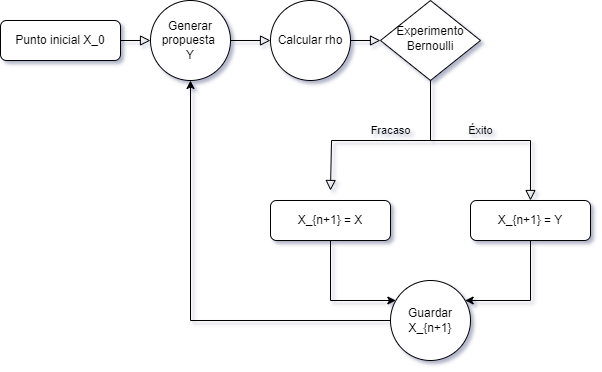
\includegraphics[width = 14 cm]{MCMC.png} 
    % \caption{}
    \label{Fig. M-H}
\end{figure} 

El algoritmo previamente esbozado a manera de opúsculo, subrepticiamente converge en distribución estacionaria a la distribución objetivo. Indudablemente dicha convergencia está asegurada por el Teorema Ergódico en cadenas de Markov (\cite{norris1998markov}). En beneficio del mencionado teorema, basta con construir una cadena de Markov de estados continuos a tiempos discretos recurrente e irreducible y aperiódica cuyo kernel de transición cumpla con balance detallado con respecto a $f(x)$. Para ahondar en detalles se requiere de un extenso estudio en cadenas de Markov a tiempo discreto con una cantidad numerable no finita de estados, donde en lugar de la usual matriz de transición se usa un operador de salto llamado kernel de transición. Un estudio completo del algoritmo de Metropolis-Hastings se encuentra en (\cite{mengersen1996rates}).

Pese a la enrevesada formalización del método, la estructura del algoritmo Metropolis-Hastings basta para dilucidar en ciertos detalles. Primeramente, del paso uno es claro que se debe elegir una distribución asociada a la variable propuesta $Y$ de forma que no sea un problema simular de esta. Además, dado que la propuesta se acepta o rechaza para ser realización de la variable $X$ asociada a la distribución objetivo, entonces se debe eligir una distribución de $Y$ tal que $supp\{X\} \subset supp\{Y\}$, que denota el soporte de la variable $Y$ debe contener el soporte de la variable objetivo $X$.

Asimismo, el segundo paso del algoritmo Metropolis-Hastings se observa la prescindencia del factor de normalización de la distribución objetivo puesto que solo es relevante el cociente $\frac{f(y)}{f(x)}$, un atributo peculiar de la distribución posterior. Paralelamente, el tercer paso del algoritmo se observa la propiedad de Markov, ya que la aceptación de la propuesta para pertenecer a la cadena depende estocásticamente del estado que lo precede unicamente.

\section{Forward map aproximado}

Hay que destacar que, una vez abordado el enfoque bayesiano para el problema inverso y el método MCMC para obtener la distribución posterior de los parámetros del modelo bajo estudio, el reto a superar recae en la implementación de la metodología descrita. Es preciso tener presente que pese a ser una metodología ampliamente funcional, no se cierra la puerta a inquerir mejoras en su procedimiento. Es por ello que la propuesta principal del trabajo de tesis es la introducción del forward map aproximado.

El forward map aproximado $F_{\theta}^{*}$ es una construcción multifacética basada en aproximaciones de estadística espacial. Tal aproximación pretende crear una distribución posterior aproximada $\tilde{\pi}(\theta|\mathbf{y})$ con la sustitución del forward map a su versión aproximada, de forma que la simulación de esta nueva distribución posterior sea más eficiente por el algoritmo Metropolis-Hastings. 

\subsection*{Construcción del forward map aproximado}
Existen diferentes maneras de hacer las aproximaciones del forward map. La forma propuesta es considerar una discretización del espacio de parámetros $\Theta$. Usando coordenadas canónicas, cada $\theta \in \Theta \subset \mathbb{R}^d$ se puede escribir como $\theta = (\theta_1, \theta_2, \cdots, \theta_d)$. Consideremos para cada coordenada un intervalo $[\theta_i^{min},\theta_i^{max}]$ para toda $i \in \{1,\cdots,d\}$, donde $\theta_i^{min}$ y $\theta_i^{max}$ son cotas para el espacio de parámetros que contenga la masa de probabilidad, puede pensarse en tomar cuantiles de $0.01$ y $0.99$ respectivamente de la distribución marginal a priori para $\theta_i$. Posteriormente, tomemos una partición equidistante en $M$ puntos para cada coordenada. Más llanamente, la partición de la coordenada $i-$ésima es el conjunto $\mathcal{M}_i =\{ \theta_i^{(1)}, \theta_i^{(2)},\cdots , \theta_i^{(M-1)}, \theta_i^{(M)}\}$ con $\theta_i^{(1)} = \theta_i^{min}$ y $\theta_i^{(M)} = \theta_i^{max}$. De esta forma, la partición crea una malla $\mathcal{M} = \mathcal{M}_1 \times \cdots \times \mathcal{M}_d$ del espacio parametral $\Theta$. Observese que la cardinalidad de $\mathcal{M}$ es de $M^d$. Denotemos por $\vartheta$ a los elementos de $\mathcal{M}$, así el enmallado se constituye de $M^d$ parámetros. Es decir, se establece que $\mathcal{M} = \{\vartheta_1, \vartheta_2, \cdots, \vartheta_{M^d}\}$, notese que $\vartheta_j \in \Theta$ para toda $j \in \{1,\cdots, M^d \}$.

Seguidamente, se requiere evaluar el forward map para cada elemento de $\mathcal{M}$, en la notación acordada se requiere $y_j = F(\vartheta_j)$, con $y_j = y_j(t)$ funciones continuas, que al estar restringidos a modelos dados por ODE es necesario un calculo intermedio. Dicho en otras palabras, solo se resuelven las ecuaciones diferenciales con los parámetros donde el enmallado interseca.

Para terminar, el forward map aproximado para parámetros $\theta \notin \mathcal{M}$ se propone buscar a los $k$ vectores de parámetros $\vartheta$ más cercanos en distancia euclideana a $\theta$, denotando estos $k$ vecinos por $\vartheta^{(1)}, \cdots, \vartheta^{(k)}$ cada uno a una distancia $d_1, \cdots, d_k$ de $\theta$, respectivamente; con $d_1 \leq d_2 \leq \dots \leq d_k$. La aproximación al forward map con $k$ vecinos en una malla con $M$ particiones es
\begin{align}
    \tilde{F}^{k}_M(\theta) = \sum_{j = 1}^{k} \omega_j F \left(\vartheta^{(j)}\right)
    \label{2.4.01}
\end{align}
donde $\omega_j = d_j^{-1}/ \sum_{i=1}^{k} d_i^{-1}$, que es una suma ponderada inversamente por las distancias, ya que se pretende que parámetros `lejanos' de $\theta$ tengan menor relevancia que los `cercanos'. 


\subsection*{Consistencia y utilidad del forward map aproximado}

La preeminencia potencial del uso del forward map aproximado para el estudio del problema inverso reside parcialmente en un menor tiempo de ejecución de la implementación en contraste con su análogo ordinario. Existen modelos de ecuaciones diferenciales cuya implementación del problema inverso bajo enfoque bayesiano toma días en ejecutarse, vease \cite{Anel}.
Debido a la reticente necesidad humana en aplicaciones impostergables es imperativo agilizar el tiempo en operación. Concisamente en modelos epidemiológicos la rapidez de acción se torna fundamental como lo fue en la predicción de ocupación hospitalaria por COVID-19 en la zona metropolitana de la CDMX (\cite{capistran2020forecasting}).

Por otro lado, fuera de las aplicaciones prácticas del método esbozado con el forward map aproximado, es de sumo interés matemático el estudio de la consistencia del método propuesto. Recordemos que tenemos espacio de maniobra para la construcción del forward map aproximado al mover la densidad de puntos en la malla $M$ así como en la cantidad de vecinos $k$ usados para la suma ponderada. De esta misma forma, tras sustituir el forward map aproximado (\ref{2.4.01}) en la expresión (\ref{2.2.04}) obtenemos la distribución posterior aproximada de los parámetros del modelo. Formalizando, salvo un factor de normalización definimos
\begin{align*}
    \tilde{\pi}^{k}_M(\theta|\mathbf{y}) \propto \left(\frac{1}{2\pi \sigma^2}\right) ^{n/2}\exp \left \{  -\frac{1}{2\sigma^2}\sum_{i = 1}^{n} \left(y_i - F^k_M(\theta)\right)^2 \right \}\pi(\theta),
\end{align*}
la distribución posterior aproximada dado las observaciones $\mathbf{y} = (y_1,\cdots, y_n)$ al tiempo $t_1, \cdots, t_n$; respectivamente. Consideremos que la aproximación a la distribución posterior usando la metodología ordinaria del problema inverso es en efecto una aproximación plausible usando la \textit{distancia de Kullback-Leibler}.

Si $f(x)$ y $g(x)$ son funciones de densidad de probabilidad. La distancia de Kullback-Leibler entre $f$ y $g$ se define como
\begin{align*}
    D(f,g) = \int f(x)\log \left(\frac{f(x)}{g(x)}\right) dx.
\end{align*}
Se puede mostrar que $D(f,g) \geq 0$ y $D(f,f) = 0$ (\cite{wasserman2006all}).
Definamos la distancia entre las distribuciones posteriores como
\begin{align*}
    c^k_M = D \left( \pi(\theta|\mathbf{y}),\tilde{\pi}^{k}_M(\theta|\mathbf{y})\right)
\end{align*}

Diremos que el forward map aproximado es \textbf{consistente} si para una cantidad de vecinos $k$ fijo y conocido, las distancias 
\begin{align*}
    c^k_M \rightarrow 0 \:\:\:\:\:\: \text{a medida que}\:\:\:\:\:\: M \rightarrow \infty
\end{align*}

En el caso de un vecino ($k = 1$) la consistencia es trivial puesto que al hacer la malla más fina, el forward map aproximado será idéntico al forward map ordinario.

El estudio para $k > 1$ requiere de una estructura teórica sobre las cualidades particulares de la ecuación diferencial del modelo en cuestión. De forma que para indagar sobre la consistencia ees necesario usar técnicas heurísticas. En el capítulo siguiente se consideran modelos paramétricos particulares aplicando las metodologías del problema inverso con y sin aproximación para así cotejar empíricamente cierto grado de convergencia.









% Esta estructura de aproximación se presta a la interpretación de que la información obtenida en mallas finas sea transmitidas a los vecinos.